Para realizar la pantalla de supervisión, control y adquisición de datos operador (SCADA) se utilizó el software iFix perteneciente al grupo General Electric.\\
En la pantalla principal se creó un esquemático tentativo del circuito hidráulico físico que se posee con las respectivas variables de presión y caudal, a las cuales se sumó variables propias del motor, otra sección se destinó a las alarmas, al control de las variables y la última al Historian (Figura \ref{fig:scada1}).

\begin{figure}[htb]
	\centering
	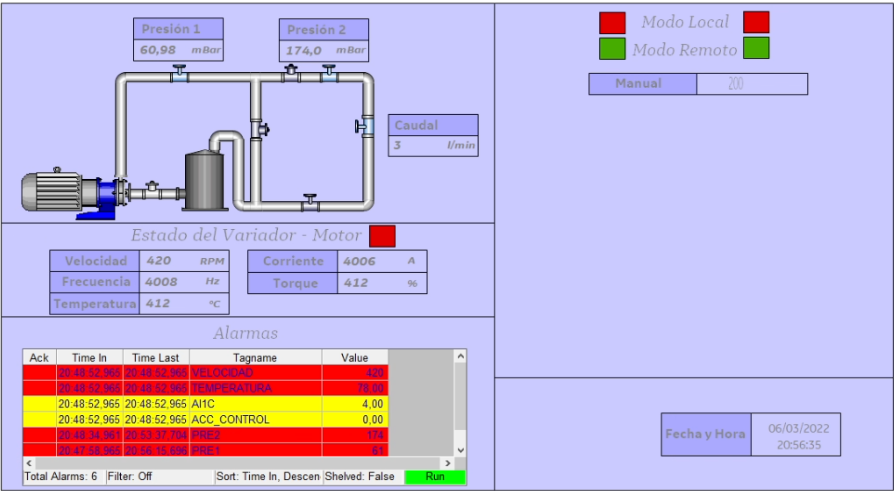
\includegraphics[scale=0.5]{scada2.png}
	\captionof{figure}{Pantalla SCADA}
	\label{fig:scada1}
\end{figure}


\subsubsection{Configuración iFix o Configuracion MBE?}
Para realizar la configuración de cada ícono con su respectiva variable se debió crear un MBE dónde se estipula la dirección y los mapas de memorias que luego serán utilizadas por el DataBase. 


\paragraph{MBE}
\subsubsection{DataBase}

\paragraph{Lista de direcciones utilizadas}
Poner lista que esta en drive
\paragraph{Pruebas mediante ModSim}
Para realizar pruebas previas a la implementación final se utilizó el programa ModSim, donde se generó los distintos mapas de memoria utilizados y allí se podían modificar variables para observarlas en el SCADA.

\begin{figure}[htb]
	\centering
	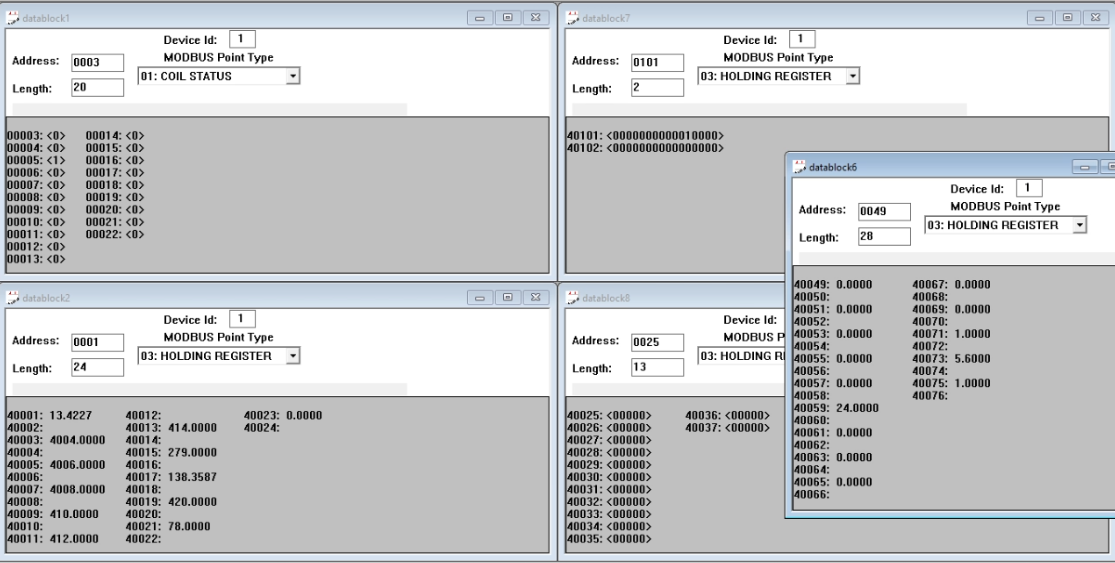
\includegraphics[scale=0.5]{modsim1.png}
	\captionof{figure}{ModSim}
	\label{fig:modsim1}
\end{figure}

\subsubsection{Distintas pantallas}


\subsection{Alarmas}
Dentro de la pantalla principal es posible observar el alarmero. Estas alarmas están compuestas por las variables de la siguiente \fcolorbox{red}{yellow}{tabla} con sus respectivos valores y prioridades.
Poner lista que esta en drive
\subsection{iHistorian}
\begin{figure}[htb]
	\centering
	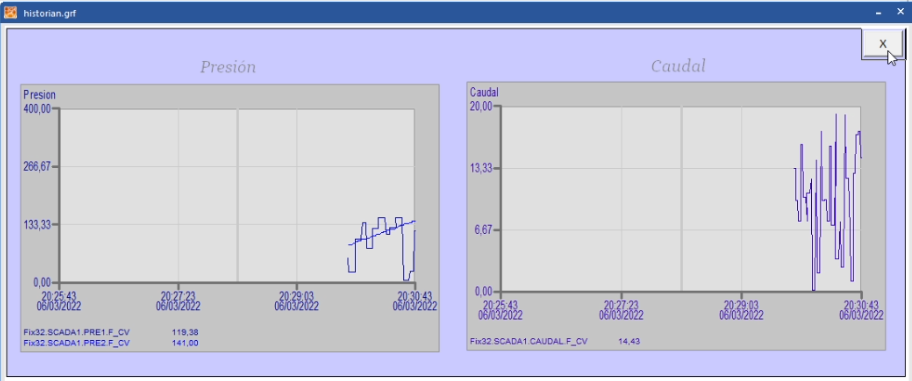
\includegraphics[scale=0.5]{scada3.png}
	\captionof{figure}{Pantalla SCADA}
	\label{fig:scada3}
\end{figure}

\subsection{Direcciones}
Poner acá las de ifix y unity? como la utilizada en drive?